\documentclass[1p]{elsarticle_modified}
%\bibliographystyle{elsarticle-num}

%\usepackage[colorlinks]{hyperref}
%\usepackage{abbrmath_seonhwa} %\Abb, \Ascr, \Acal ,\Abf, \Afrak
\usepackage{amsfonts}
\usepackage{amssymb}
\usepackage{amsmath}
\usepackage{amsthm}
\usepackage{scalefnt}
\usepackage{amsbsy}
\usepackage{kotex}
\usepackage{caption}
\usepackage{subfig}
\usepackage{color}
\usepackage{graphicx}
\usepackage{xcolor} %% white, black, red, green, blue, cyan, magenta, yellow
\usepackage{float}
\usepackage{setspace}
\usepackage{hyperref}

\usepackage{tikz}
\usetikzlibrary{arrows}

\usepackage{multirow}
\usepackage{array} % fixed length table
\usepackage{hhline}

%%%%%%%%%%%%%%%%%%%%%
\makeatletter
\renewcommand*\env@matrix[1][\arraystretch]{%
	\edef\arraystretch{#1}%
	\hskip -\arraycolsep
	\let\@ifnextchar\new@ifnextchar
	\array{*\c@MaxMatrixCols c}}
\makeatother %https://tex.stackexchange.com/questions/14071/how-can-i-increase-the-line-spacing-in-a-matrix
%%%%%%%%%%%%%%%

\usepackage[normalem]{ulem}

\newcommand{\msout}[1]{\ifmmode\text{\sout{\ensuremath{#1}}}\else\sout{#1}\fi}
%SOURCE: \msout is \stkout macro in https://tex.stackexchange.com/questions/20609/strikeout-in-math-mode

\newcommand{\cancel}[1]{
	\ifmmode
	{\color{red}\msout{#1}}
	\else
	{\color{red}\sout{#1}}
	\fi
}

\newcommand{\add}[1]{
	{\color{blue}\uwave{#1}}
}

\newcommand{\replace}[2]{
	\ifmmode
	{\color{red}\msout{#1}}{\color{blue}\uwave{#2}}
	\else
	{\color{red}\sout{#1}}{\color{blue}\uwave{#2}}
	\fi
}

\newcommand{\Sol}{\mathcal{S}} %segment
\newcommand{\D}{D} %diagram
\newcommand{\A}{\mathcal{A}} %arc


%%%%%%%%%%%%%%%%%%%%%%%%%%%%%5 test

\def\sl{\operatorname{\textup{SL}}(2,\Cbb)}
\def\psl{\operatorname{\textup{PSL}}(2,\Cbb)}
\def\quan{\mkern 1mu \triangleright \mkern 1mu}

\theoremstyle{definition}
\newtheorem{thm}{Theorem}[section]
\newtheorem{prop}[thm]{Proposition}
\newtheorem{lem}[thm]{Lemma}
\newtheorem{ques}[thm]{Question}
\newtheorem{cor}[thm]{Corollary}
\newtheorem{defn}[thm]{Definition}
\newtheorem{exam}[thm]{Example}
\newtheorem{rmk}[thm]{Remark}
\newtheorem{alg}[thm]{Algorithm}

\newcommand{\I}{\sqrt{-1}}
\begin{document}

%\begin{frontmatter}
%
%\title{Boundary parabolic representations of knots up to 8 crossings}
%
%%% Group authors per affiliation:
%\author{Yunhi Cho} 
%\address{Department of Mathematics, University of Seoul, Seoul, Korea}
%\ead{yhcho@uos.ac.kr}
%
%
%\author{Seonhwa Kim} %\fnref{s_kim}}
%\address{Center for Geometry and Physics, Institute for Basic Science, Pohang, 37673, Korea}
%\ead{ryeona17@ibs.re.kr}
%
%\author{Hyuk Kim}
%\address{Department of Mathematical Sciences, Seoul National University, Seoul 08826, Korea}
%\ead{hyukkim@snu.ac.kr}
%
%\author{Seokbeom Yoon}
%\address{Department of Mathematical Sciences, Seoul National University, Seoul, 08826,  Korea}
%\ead{sbyoon15@snu.ac.kr}
%
%\begin{abstract}
%We find all boundary parabolic representation of knots up to 8 crossings.
%
%\end{abstract}
%\begin{keyword}
%    \MSC[2010] 57M25 
%\end{keyword}
%
%\end{frontmatter}

%\linenumbers
%\tableofcontents
%
\newcommand\colored[1]{\textcolor{white}{\rule[-0.35ex]{0.8em}{1.4ex}}\kern-0.8em\color{red} #1}%
%\newcommand\colored[1]{\textcolor{white}{ #1}\kern-2.17ex	\textcolor{white}{ #1}\kern-1.81ex	\textcolor{white}{ #1}\kern-2.15ex\color{red}#1	}

{\Large $\underline{12a_{0715}~(K12a_{0715})}$}

\setlength{\tabcolsep}{10pt}
\renewcommand{\arraystretch}{1.6}
\vspace{1cm}\begin{tabular}{m{100pt}>{\centering\arraybackslash}m{274pt}}
\multirow{5}{120pt}{
	\centering
	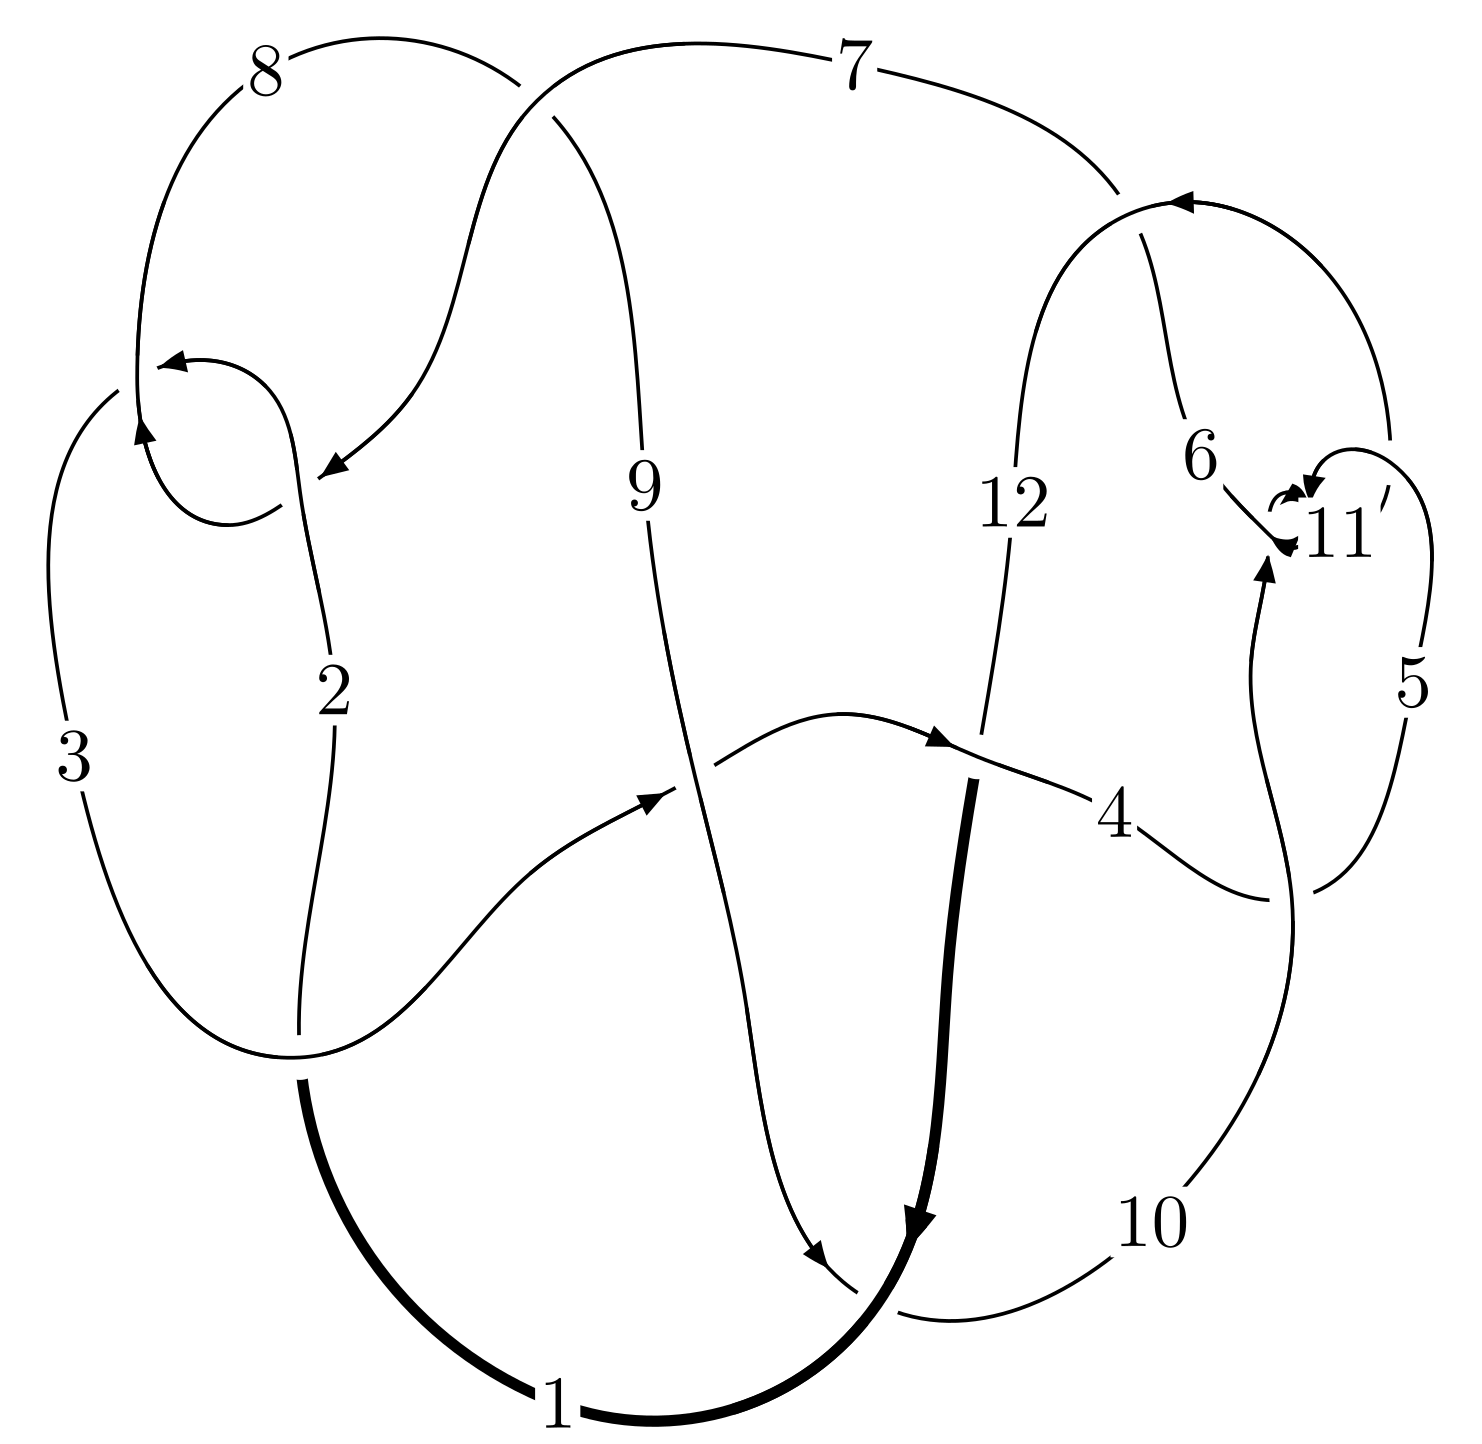
\includegraphics[width=112pt]{../../../GIT/diagram.site/Diagrams/png/1516_12a_0715.png}\\
\ \ \ A knot diagram\footnotemark}&
\allowdisplaybreaks
\textbf{Linearized knot diagam} \\
\cline{2-2}
 &
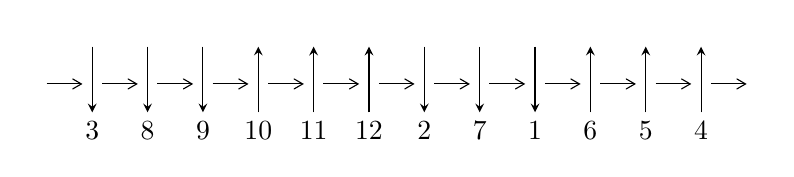
\begin{tikzpicture}[x=20pt, y=17pt]
	% nodes
	\node (C0) at (0, 0) {};
	\node (C1) at (1, 0) {};
	\node (C1U) at (1, +1) {};
	\node (C1D) at (1, -1) {3};

	\node (C2) at (2, 0) {};
	\node (C2U) at (2, +1) {};
	\node (C2D) at (2, -1) {8};

	\node (C3) at (3, 0) {};
	\node (C3U) at (3, +1) {};
	\node (C3D) at (3, -1) {9};

	\node (C4) at (4, 0) {};
	\node (C4U) at (4, +1) {};
	\node (C4D) at (4, -1) {10};

	\node (C5) at (5, 0) {};
	\node (C5U) at (5, +1) {};
	\node (C5D) at (5, -1) {11};

	\node (C6) at (6, 0) {};
	\node (C6U) at (6, +1) {};
	\node (C6D) at (6, -1) {12};

	\node (C7) at (7, 0) {};
	\node (C7U) at (7, +1) {};
	\node (C7D) at (7, -1) {2};

	\node (C8) at (8, 0) {};
	\node (C8U) at (8, +1) {};
	\node (C8D) at (8, -1) {7};

	\node (C9) at (9, 0) {};
	\node (C9U) at (9, +1) {};
	\node (C9D) at (9, -1) {1};

	\node (C10) at (10, 0) {};
	\node (C10U) at (10, +1) {};
	\node (C10D) at (10, -1) {6};

	\node (C11) at (11, 0) {};
	\node (C11U) at (11, +1) {};
	\node (C11D) at (11, -1) {5};

	\node (C12) at (12, 0) {};
	\node (C12U) at (12, +1) {};
	\node (C12D) at (12, -1) {4};
	\node (C13) at (13, 0) {};

	% arrows
	\draw[->,>={angle 60}]
	(C0) edge (C1) (C1) edge (C2) (C2) edge (C3) (C3) edge (C4) (C4) edge (C5) (C5) edge (C6) (C6) edge (C7) (C7) edge (C8) (C8) edge (C9) (C9) edge (C10) (C10) edge (C11) (C11) edge (C12) (C12) edge (C13) ;	\draw[->,>=stealth]
	(C1U) edge (C1D) (C2U) edge (C2D) (C3U) edge (C3D) (C4D) edge (C4U) (C5D) edge (C5U) (C6D) edge (C6U) (C7U) edge (C7D) (C8U) edge (C8D) (C9U) edge (C9D) (C10D) edge (C10U) (C11D) edge (C11U) (C12D) edge (C12U) ;
	\end{tikzpicture} \\
\hhline{~~} \\& 
\textbf{Solving Sequence} \\ \cline{2-2} 
 &
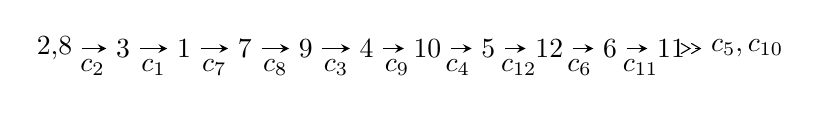
\begin{tikzpicture}[x=22pt, y=7pt]
	% node
	\node (A0) at (-1/8, 0) {2,8};
	\node (A1) at (1, 0) {3};
	\node (A2) at (2, 0) {1};
	\node (A3) at (3, 0) {7};
	\node (A4) at (4, 0) {9};
	\node (A5) at (5, 0) {4};
	\node (A6) at (6, 0) {10};
	\node (A7) at (7, 0) {5};
	\node (A8) at (8, 0) {12};
	\node (A9) at (9, 0) {6};
	\node (A10) at (10, 0) {11};
	\node (C1) at (1/2, -1) {$c_{2}$};
	\node (C2) at (3/2, -1) {$c_{1}$};
	\node (C3) at (5/2, -1) {$c_{7}$};
	\node (C4) at (7/2, -1) {$c_{8}$};
	\node (C5) at (9/2, -1) {$c_{3}$};
	\node (C6) at (11/2, -1) {$c_{9}$};
	\node (C7) at (13/2, -1) {$c_{4}$};
	\node (C8) at (15/2, -1) {$c_{12}$};
	\node (C9) at (17/2, -1) {$c_{6}$};
	\node (C10) at (19/2, -1) {$c_{11}$};
	\node (A11) at (45/4, 0) {$c_{5},c_{10}$};

	% edge
	\draw[->,>=stealth]	
	(A0) edge (A1) (A1) edge (A2) (A2) edge (A3) (A3) edge (A4) (A4) edge (A5) (A5) edge (A6) (A6) edge (A7) (A7) edge (A8) (A8) edge (A9) (A9) edge (A10) ;
	\draw[->>,>={angle 60}]	
	(A10) edge (A11);
\end{tikzpicture} \\ 

\end{tabular} \\

\footnotetext{
The image of knot diagram is generated by the software ``\textbf{Draw programme}" developed by Andrew Bartholomew(\url{http://www.layer8.co.uk/maths/draw/index.htm\#Running-draw}), where we modified some parts for our purpose(\url{https://github.com/CATsTAILs/LinksPainter}).
}\phantom \\ \newline 
\centering \textbf{Ideals for irreducible components\footnotemark of $X_{\text{par}}$} 
 
\begin{align*}
I^u_{1}&=\langle 
u^{84}+u^{83}+\cdots+2 u+1\rangle \\
\\
\end{align*}
\raggedright * 1 irreducible components of $\dim_{\mathbb{C}}=0$, with total 84 representations.\\
\footnotetext{All coefficients of polynomials are rational numbers. But the coefficients are sometimes approximated in decimal forms when there is not enough margin.}
\newpage
\renewcommand{\arraystretch}{1}
\centering \section*{I. $I^u_{1}= \langle u^{84}+u^{83}+\cdots+2 u+1 \rangle$}
\flushleft \textbf{(i) Arc colorings}\\
\begin{tabular}{m{7pt} m{180pt} m{7pt} m{180pt} }
\flushright $a_{2}=$&$\begin{pmatrix}1\\0\end{pmatrix}$ \\
\flushright $a_{8}=$&$\begin{pmatrix}0\\u\end{pmatrix}$ \\
\flushright $a_{3}=$&$\begin{pmatrix}1\\u^2\end{pmatrix}$ \\
\flushright $a_{1}=$&$\begin{pmatrix}- u^2+1\\- u^4\end{pmatrix}$ \\
\flushright $a_{7}=$&$\begin{pmatrix}u\\u\end{pmatrix}$ \\
\flushright $a_{9}=$&$\begin{pmatrix}- u^3\\- u^3+u\end{pmatrix}$ \\
\flushright $a_{4}=$&$\begin{pmatrix}- u^8+u^6- u^4+1\\- u^8+2 u^6-2 u^4+2 u^2\end{pmatrix}$ \\
\flushright $a_{10}=$&$\begin{pmatrix}- u^9+2 u^7-3 u^5+2 u^3- u\\- u^{11}+u^9-2 u^7+u^5- u^3+u\end{pmatrix}$ \\
\flushright $a_{5}=$&$\begin{pmatrix}u^{28}-5 u^{26}+\cdots+u^2+1\\u^{30}-4 u^{28}+\cdots-2 u^4+u^2\end{pmatrix}$ \\
\flushright $a_{12}=$&$\begin{pmatrix}u^{20}-3 u^{18}+7 u^{16}-10 u^{14}+10 u^{12}-7 u^{10}+u^8+2 u^6-3 u^4+u^2+1\\u^{20}-4 u^{18}+10 u^{16}-18 u^{14}+23 u^{12}-24 u^{10}+18 u^8-10 u^6+3 u^4\end{pmatrix}$ \\
\flushright $a_{6}=$&$\begin{pmatrix}- u^{39}+6 u^{37}+\cdots+8 u^5-2 u^3\\- u^{39}+7 u^{37}+\cdots-3 u^5+u\end{pmatrix}$ \\
\flushright $a_{11}=$&$\begin{pmatrix}u^{78}-13 u^{76}+\cdots+2 u^2+1\\u^{80}-12 u^{78}+\cdots-16 u^6+4 u^4\end{pmatrix}$\\&\end{tabular}
\flushleft \textbf{(ii) Obstruction class $= -1$}\\~\\
\flushleft \textbf{(iii) Cusp Shapes $= -4 u^{83}+56 u^{81}+\cdots-16 u-6$}\\~\\
\newpage\renewcommand{\arraystretch}{1}
\flushleft \textbf{(iv) u-Polynomials at the component}\newline \\
\begin{tabular}{m{50pt}|m{274pt}}
Crossings & \hspace{64pt}u-Polynomials at each crossing \\
\hline $$\begin{aligned}c_{1},c_{8}\end{aligned}$$&$\begin{aligned}
&u^{84}+27 u^{83}+\cdots-2 u+1
\end{aligned}$\\
\hline $$\begin{aligned}c_{2},c_{7}\end{aligned}$$&$\begin{aligned}
&u^{84}+u^{83}+\cdots+2 u+1
\end{aligned}$\\
\hline $$\begin{aligned}c_{3}\end{aligned}$$&$\begin{aligned}
&u^{84}- u^{83}+\cdots-4 u+1
\end{aligned}$\\
\hline $$\begin{aligned}c_{4},c_{6}\end{aligned}$$&$\begin{aligned}
&u^{84}+u^{83}+\cdots+126 u+37
\end{aligned}$\\
\hline $$\begin{aligned}c_{5},c_{10},c_{11}\end{aligned}$$&$\begin{aligned}
&u^{84}- u^{83}+\cdots+u^2+1
\end{aligned}$\\
\hline $$\begin{aligned}c_{9}\end{aligned}$$&$\begin{aligned}
&u^{84}+7 u^{83}+\cdots+36022 u+4921
\end{aligned}$\\
\hline $$\begin{aligned}c_{12}\end{aligned}$$&$\begin{aligned}
&u^{84}+7 u^{83}+\cdots+24 u+1
\end{aligned}$\\
\hline
\end{tabular}\\~\\
\newpage\renewcommand{\arraystretch}{1}
\flushleft \textbf{(v) Riley Polynomials at the component}\newline \\
\begin{tabular}{m{50pt}|m{274pt}}
Crossings & \hspace{64pt}Riley Polynomials at each crossing \\
\hline $$\begin{aligned}c_{1},c_{8}\end{aligned}$$&$\begin{aligned}
&y^{84}+61 y^{83}+\cdots-14 y+1
\end{aligned}$\\
\hline $$\begin{aligned}c_{2},c_{7}\end{aligned}$$&$\begin{aligned}
&y^{84}-27 y^{83}+\cdots+2 y+1
\end{aligned}$\\
\hline $$\begin{aligned}c_{3}\end{aligned}$$&$\begin{aligned}
&y^{84}+y^{83}+\cdots+18 y+1
\end{aligned}$\\
\hline $$\begin{aligned}c_{4},c_{6}\end{aligned}$$&$\begin{aligned}
&y^{84}-55 y^{83}+\cdots+22678 y+1369
\end{aligned}$\\
\hline $$\begin{aligned}c_{5},c_{10},c_{11}\end{aligned}$$&$\begin{aligned}
&y^{84}+69 y^{83}+\cdots+2 y+1
\end{aligned}$\\
\hline $$\begin{aligned}c_{9}\end{aligned}$$&$\begin{aligned}
&y^{84}+29 y^{83}+\cdots+233801190 y+24216241
\end{aligned}$\\
\hline $$\begin{aligned}c_{12}\end{aligned}$$&$\begin{aligned}
&y^{84}+y^{83}+\cdots+154 y+1
\end{aligned}$\\
\hline
\end{tabular}\\~\\
\newpage\flushleft \textbf{(vi) Complex Volumes and Cusp Shapes}
$$\begin{array}{c|c|c}  
\text{Solutions to }I^u_{1}& \I (\text{vol} + \sqrt{-1}CS) & \text{Cusp shape}\\
 \hline 
\begin{aligned}
u &= \phantom{-}1.000680 + 0.114921 I\end{aligned}
 & -3.30654 - 2.82803 I & \phantom{-0.000000 } 0 \\ \hline\begin{aligned}
u &= \phantom{-}1.000680 - 0.114921 I\end{aligned}
 & -3.30654 + 2.82803 I & \phantom{-0.000000 } 0 \\ \hline\begin{aligned}
u &= -0.905164 + 0.455365 I\end{aligned}
 & -2.33728 - 4.40675 I & \phantom{-0.000000 } 0 \\ \hline\begin{aligned}
u &= -0.905164 - 0.455365 I\end{aligned}
 & -2.33728 + 4.40675 I & \phantom{-0.000000 } 0 \\ \hline\begin{aligned}
u &= -0.974058 + 0.042964 I\end{aligned}
 & -2.08693 + 0.08784 I & \phantom{-0.000000 } 0 \\ \hline\begin{aligned}
u &= -0.974058 - 0.042964 I\end{aligned}
 & -2.08693 - 0.08784 I & \phantom{-0.000000 } 0 \\ \hline\begin{aligned}
u &= -0.694407 + 0.683449 I\end{aligned}
 & -1.36007 + 2.80367 I & \phantom{-0.000000 } 0 \\ \hline\begin{aligned}
u &= -0.694407 - 0.683449 I\end{aligned}
 & -1.36007 - 2.80367 I & \phantom{-0.000000 } 0 \\ \hline\begin{aligned}
u &= \phantom{-}1.027590 + 0.043282 I\end{aligned}
 & -6.59695 + 3.00636 I & \phantom{-0.000000 } 0 \\ \hline\begin{aligned}
u &= \phantom{-}1.027590 - 0.043282 I\end{aligned}
 & -6.59695 - 3.00636 I & \phantom{-0.000000 } 0 \\ \hline\begin{aligned}
u &= \phantom{-}1.018280 + 0.162257 I\end{aligned}
 & -2.47637 - 2.14319 I & \phantom{-0.000000 } 0 \\ \hline\begin{aligned}
u &= \phantom{-}1.018280 - 0.162257 I\end{aligned}
 & -2.47637 + 2.14319 I & \phantom{-0.000000 } 0 \\ \hline\begin{aligned}
u &= \phantom{-}0.853648 + 0.436783 I\end{aligned}
 & \phantom{-}2.14949 + 0.51882 I & \phantom{-0.000000 } 0 \\ \hline\begin{aligned}
u &= \phantom{-}0.853648 - 0.436783 I\end{aligned}
 & \phantom{-}2.14949 - 0.51882 I & \phantom{-0.000000 } 0 \\ \hline\begin{aligned}
u &= \phantom{-}0.685516 + 0.786962 I\end{aligned}
 & -3.09599 + 3.71420 I & \phantom{-0.000000 } 0 \\ \hline\begin{aligned}
u &= \phantom{-}0.685516 - 0.786962 I\end{aligned}
 & -3.09599 - 3.71420 I & \phantom{-0.000000 } 0 \\ \hline\begin{aligned}
u &= -1.038020 + 0.108768 I\end{aligned}
 & -9.19499 + 3.72935 I & \phantom{-0.000000 } 0 \\ \hline\begin{aligned}
u &= -1.038020 - 0.108768 I\end{aligned}
 & -9.19499 - 3.72935 I & \phantom{-0.000000 } 0 \\ \hline\begin{aligned}
u &= -1.036400 + 0.157863 I\end{aligned}
 & \phantom{-}0.57258 + 6.20944 I & \phantom{-0.000000 } 0 \\ \hline\begin{aligned}
u &= -1.036400 - 0.157863 I\end{aligned}
 & \phantom{-}0.57258 - 6.20944 I & \phantom{-0.000000 } 0 \\ \hline\begin{aligned}
u &= \phantom{-}1.046330 + 0.154384 I\end{aligned}
 & -4.03349 - 10.29500 I & \phantom{-0.000000 } 0 \\ \hline\begin{aligned}
u &= \phantom{-}1.046330 - 0.154384 I\end{aligned}
 & -4.03349 + 10.29500 I & \phantom{-0.000000 } 0 \\ \hline\begin{aligned}
u &= -0.712204 + 0.784436 I\end{aligned}
 & \phantom{-}2.71266 - 2.44286 I & \phantom{-0.000000 } 0 \\ \hline\begin{aligned}
u &= -0.712204 - 0.784436 I\end{aligned}
 & \phantom{-}2.71266 + 2.44286 I & \phantom{-0.000000 } 0 \\ \hline\begin{aligned}
u &= \phantom{-}0.739410 + 0.760668 I\end{aligned}
 & \phantom{-}3.28834 - 0.55550 I & \phantom{-0.000000 } 0 \\ \hline\begin{aligned}
u &= \phantom{-}0.739410 - 0.760668 I\end{aligned}
 & \phantom{-}3.28834 + 0.55550 I & \phantom{-0.000000 } 0 \\ \hline\begin{aligned}
u &= -0.896150 + 0.594563 I\end{aligned}
 & -0.81662 + 2.30924 I & \phantom{-0.000000 } 0 \\ \hline\begin{aligned}
u &= -0.896150 - 0.594563 I\end{aligned}
 & -0.81662 - 2.30924 I & \phantom{-0.000000 } 0 \\ \hline\begin{aligned}
u &= -0.696784 + 0.820077 I\end{aligned}
 & \phantom{-}2.51894 - 10.14580 I & \phantom{-0.000000 } 0 \\ \hline\begin{aligned}
u &= -0.696784 - 0.820077 I\end{aligned}
 & \phantom{-}2.51894 + 10.14580 I & \phantom{-0.000000 } 0\\
 \hline 
 \end{array}$$\newpage$$\begin{array}{c|c|c}  
\text{Solutions to }I^u_{1}& \I (\text{vol} + \sqrt{-1}CS) & \text{Cusp shape}\\
 \hline 
\begin{aligned}
u &= \phantom{-}0.702760 + 0.818077 I\end{aligned}
 & \phantom{-}7.10746 + 5.96437 I & \phantom{-0.000000 } 0 \\ \hline\begin{aligned}
u &= \phantom{-}0.702760 - 0.818077 I\end{aligned}
 & \phantom{-}7.10746 - 5.96437 I & \phantom{-0.000000 } 0 \\ \hline\begin{aligned}
u &= -0.711331 + 0.814103 I\end{aligned}
 & \phantom{-}4.01224 - 1.74526 I & \phantom{-0.000000 } 0 \\ \hline\begin{aligned}
u &= -0.711331 - 0.814103 I\end{aligned}
 & \phantom{-}4.01224 + 1.74526 I & \phantom{-0.000000 } 0 \\ \hline\begin{aligned}
u &= -0.839981 + 0.681059 I\end{aligned}
 & -1.13918 + 2.62448 I & \phantom{-0.000000 } 0 \\ \hline\begin{aligned}
u &= -0.839981 - 0.681059 I\end{aligned}
 & -1.13918 - 2.62448 I & \phantom{-0.000000 } 0 \\ \hline\begin{aligned}
u &= \phantom{-}0.938413 + 0.554154 I\end{aligned}
 & -6.71108 - 2.02254 I & \phantom{-0.000000 } 0 \\ \hline\begin{aligned}
u &= \phantom{-}0.938413 - 0.554154 I\end{aligned}
 & -6.71108 + 2.02254 I & \phantom{-0.000000 } 0 \\ \hline\begin{aligned}
u &= -0.842956 + 0.308678 I\end{aligned}
 & -1.24656 + 3.23995 I & -1.88607 - 4.84912 I \\ \hline\begin{aligned}
u &= -0.842956 - 0.308678 I\end{aligned}
 & -1.24656 - 3.23995 I & -1.88607 + 4.84912 I \\ \hline\begin{aligned}
u &= \phantom{-}0.777185 + 0.798350 I\end{aligned}
 & \phantom{-}5.15367 + 1.34157 I & \phantom{-0.000000 } 0 \\ \hline\begin{aligned}
u &= \phantom{-}0.777185 - 0.798350 I\end{aligned}
 & \phantom{-}5.15367 - 1.34157 I & \phantom{-0.000000 } 0 \\ \hline\begin{aligned}
u &= -0.788473 + 0.795791 I\end{aligned}
 & \phantom{-}8.60971 + 2.86537 I & \phantom{-0.000000 } 0 \\ \hline\begin{aligned}
u &= -0.788473 - 0.795791 I\end{aligned}
 & \phantom{-}8.60971 - 2.86537 I & \phantom{-0.000000 } 0 \\ \hline\begin{aligned}
u &= \phantom{-}0.797824 + 0.793842 I\end{aligned}
 & \phantom{-}4.29016 - 7.05239 I & \phantom{-0.000000 } 0 \\ \hline\begin{aligned}
u &= \phantom{-}0.797824 - 0.793842 I\end{aligned}
 & \phantom{-}4.29016 + 7.05239 I & \phantom{-0.000000 } 0 \\ \hline\begin{aligned}
u &= \phantom{-}0.953308 + 0.626952 I\end{aligned}
 & \phantom{-}1.33534 - 5.16055 I & \phantom{-0.000000 } 0 \\ \hline\begin{aligned}
u &= \phantom{-}0.953308 - 0.626952 I\end{aligned}
 & \phantom{-}1.33534 + 5.16055 I & \phantom{-0.000000 } 0 \\ \hline\begin{aligned}
u &= -0.969589 + 0.611792 I\end{aligned}
 & -3.26007 + 8.69634 I & \phantom{-0.000000 } 0 \\ \hline\begin{aligned}
u &= -0.969589 - 0.611792 I\end{aligned}
 & -3.26007 - 8.69634 I & \phantom{-0.000000 } 0 \\ \hline\begin{aligned}
u &= -0.981582 + 0.680099 I\end{aligned}
 & -2.20981 + 2.51113 I & \phantom{-0.000000 } 0 \\ \hline\begin{aligned}
u &= -0.981582 - 0.680099 I\end{aligned}
 & -2.20981 - 2.51113 I & \phantom{-0.000000 } 0 \\ \hline\begin{aligned}
u &= \phantom{-}0.942272 + 0.750733 I\end{aligned}
 & \phantom{-}3.84490 + 1.24185 I & \phantom{-0.000000 } 0 \\ \hline\begin{aligned}
u &= \phantom{-}0.942272 - 0.750733 I\end{aligned}
 & \phantom{-}3.84490 - 1.24185 I & \phantom{-0.000000 } 0 \\ \hline\begin{aligned}
u &= \phantom{-}0.973775 + 0.709890 I\end{aligned}
 & \phantom{-}2.57173 - 5.03263 I & \phantom{-0.000000 } 0 \\ \hline\begin{aligned}
u &= \phantom{-}0.973775 - 0.709890 I\end{aligned}
 & \phantom{-}2.57173 + 5.03263 I & \phantom{-0.000000 } 0 \\ \hline\begin{aligned}
u &= -0.950090 + 0.748512 I\end{aligned}
 & \phantom{-}8.11226 + 2.94426 I & \phantom{-0.000000 } 0 \\ \hline\begin{aligned}
u &= -0.950090 - 0.748512 I\end{aligned}
 & \phantom{-}8.11226 - 2.94426 I & \phantom{-0.000000 } 0 \\ \hline\begin{aligned}
u &= \phantom{-}0.616499 + 0.492783 I\end{aligned}
 & \phantom{-}2.15550 + 0.43358 I & \phantom{-}3.37103 - 0.17478 I \\ \hline\begin{aligned}
u &= \phantom{-}0.616499 - 0.492783 I\end{aligned}
 & \phantom{-}2.15550 - 0.43358 I & \phantom{-}3.37103 + 0.17478 I\\
 \hline 
 \end{array}$$\newpage$$\begin{array}{c|c|c}  
\text{Solutions to }I^u_{1}& \I (\text{vol} + \sqrt{-1}CS) & \text{Cusp shape}\\
 \hline 
\begin{aligned}
u &= \phantom{-}0.958896 + 0.746173 I\end{aligned}
 & \phantom{-}4.59540 - 7.15142 I & \phantom{-0.000000 } 0 \\ \hline\begin{aligned}
u &= \phantom{-}0.958896 - 0.746173 I\end{aligned}
 & \phantom{-}4.59540 + 7.15142 I & \phantom{-0.000000 } 0 \\ \hline\begin{aligned}
u &= -0.993122 + 0.716813 I\end{aligned}
 & \phantom{-}1.86003 + 8.11878 I & \phantom{-0.000000 } 0 \\ \hline\begin{aligned}
u &= -0.993122 - 0.716813 I\end{aligned}
 & \phantom{-}1.86003 - 8.11878 I & \phantom{-0.000000 } 0 \\ \hline\begin{aligned}
u &= \phantom{-}1.005760 + 0.710135 I\end{aligned}
 & -4.06219 - 9.37250 I & \phantom{-0.000000 } 0 \\ \hline\begin{aligned}
u &= \phantom{-}1.005760 - 0.710135 I\end{aligned}
 & -4.06219 + 9.37250 I & \phantom{-0.000000 } 0 \\ \hline\begin{aligned}
u &= -1.003120 + 0.730563 I\end{aligned}
 & \phantom{-}3.12182 + 7.54780 I & \phantom{-0.000000 } 0 \\ \hline\begin{aligned}
u &= -1.003120 - 0.730563 I\end{aligned}
 & \phantom{-}3.12182 - 7.54780 I & \phantom{-0.000000 } 0 \\ \hline\begin{aligned}
u &= \phantom{-}1.008780 + 0.729448 I\end{aligned}
 & \phantom{-}6.17424 - 11.77370 I & \phantom{-0.000000 } 0 \\ \hline\begin{aligned}
u &= \phantom{-}1.008780 - 0.729448 I\end{aligned}
 & \phantom{-}6.17424 + 11.77370 I & \phantom{-0.000000 } 0 \\ \hline\begin{aligned}
u &= -1.012300 + 0.728181 I\end{aligned}
 & \phantom{-}1.5573 + 15.9558 I & \phantom{-0.000000 } 0 \\ \hline\begin{aligned}
u &= -1.012300 - 0.728181 I\end{aligned}
 & \phantom{-}1.5573 - 15.9558 I & \phantom{-0.000000 } 0 \\ \hline\begin{aligned}
u &= -0.497524 + 0.528030 I\end{aligned}
 & -2.16401 - 4.06838 I & -1.45615 + 2.43017 I \\ \hline\begin{aligned}
u &= -0.497524 - 0.528030 I\end{aligned}
 & -2.16401 + 4.06838 I & -1.45615 - 2.43017 I \\ \hline\begin{aligned}
u &= -0.151272 + 0.620418 I\end{aligned}
 & -0.20052 + 7.91026 I & \phantom{-}2.01559 - 6.55266 I \\ \hline\begin{aligned}
u &= -0.151272 - 0.620418 I\end{aligned}
 & -0.20052 - 7.91026 I & \phantom{-}2.01559 + 6.55266 I \\ \hline\begin{aligned}
u &= \phantom{-}0.131937 + 0.610074 I\end{aligned}
 & \phantom{-}4.29748 - 3.82525 I & \phantom{-}6.98451 + 4.41441 I \\ \hline\begin{aligned}
u &= \phantom{-}0.131937 - 0.610074 I\end{aligned}
 & \phantom{-}4.29748 + 3.82525 I & \phantom{-}6.98451 - 4.41441 I \\ \hline\begin{aligned}
u &= -0.101127 + 0.596695 I\end{aligned}
 & \phantom{-}1.070480 - 0.240163 I & \phantom{-}4.08415 - 0.33242 I \\ \hline\begin{aligned}
u &= -0.101127 - 0.596695 I\end{aligned}
 & \phantom{-}1.070480 + 0.240163 I & \phantom{-}4.08415 + 0.33242 I \\ \hline\begin{aligned}
u &= \phantom{-}0.247307 + 0.537464 I\end{aligned}
 & -5.22517 - 1.87101 I & -3.27342 + 3.75201 I \\ \hline\begin{aligned}
u &= \phantom{-}0.247307 - 0.537464 I\end{aligned}
 & -5.22517 + 1.87101 I & -3.27342 - 3.75201 I \\ \hline\begin{aligned}
u &= -0.130530 + 0.452424 I\end{aligned}
 & \phantom{-}0.151301 + 1.049580 I & \phantom{-}2.45407 - 6.37188 I \\ \hline\begin{aligned}
u &= -0.130530 - 0.452424 I\end{aligned}
 & \phantom{-}0.151301 - 1.049580 I & \phantom{-}2.45407 + 6.37188 I\\
 \hline 
 \end{array}$$\newpage
\newpage\renewcommand{\arraystretch}{1}
\centering \section*{ II. u-Polynomials}
\begin{tabular}{m{50pt}|m{274pt}}
Crossings & \hspace{64pt}u-Polynomials at each crossing \\
\hline $$\begin{aligned}c_{1},c_{8}\end{aligned}$$&$\begin{aligned}
&u^{84}+27 u^{83}+\cdots-2 u+1
\end{aligned}$\\
\hline $$\begin{aligned}c_{2},c_{7}\end{aligned}$$&$\begin{aligned}
&u^{84}+u^{83}+\cdots+2 u+1
\end{aligned}$\\
\hline $$\begin{aligned}c_{3}\end{aligned}$$&$\begin{aligned}
&u^{84}- u^{83}+\cdots-4 u+1
\end{aligned}$\\
\hline $$\begin{aligned}c_{4},c_{6}\end{aligned}$$&$\begin{aligned}
&u^{84}+u^{83}+\cdots+126 u+37
\end{aligned}$\\
\hline $$\begin{aligned}c_{5},c_{10},c_{11}\end{aligned}$$&$\begin{aligned}
&u^{84}- u^{83}+\cdots+u^2+1
\end{aligned}$\\
\hline $$\begin{aligned}c_{9}\end{aligned}$$&$\begin{aligned}
&u^{84}+7 u^{83}+\cdots+36022 u+4921
\end{aligned}$\\
\hline $$\begin{aligned}c_{12}\end{aligned}$$&$\begin{aligned}
&u^{84}+7 u^{83}+\cdots+24 u+1
\end{aligned}$\\
\hline
\end{tabular}\newpage\renewcommand{\arraystretch}{1}
\centering \section*{ III. Riley Polynomials}
\begin{tabular}{m{50pt}|m{274pt}}
Crossings & \hspace{64pt}Riley Polynomials at each crossing \\
\hline $$\begin{aligned}c_{1},c_{8}\end{aligned}$$&$\begin{aligned}
&y^{84}+61 y^{83}+\cdots-14 y+1
\end{aligned}$\\
\hline $$\begin{aligned}c_{2},c_{7}\end{aligned}$$&$\begin{aligned}
&y^{84}-27 y^{83}+\cdots+2 y+1
\end{aligned}$\\
\hline $$\begin{aligned}c_{3}\end{aligned}$$&$\begin{aligned}
&y^{84}+y^{83}+\cdots+18 y+1
\end{aligned}$\\
\hline $$\begin{aligned}c_{4},c_{6}\end{aligned}$$&$\begin{aligned}
&y^{84}-55 y^{83}+\cdots+22678 y+1369
\end{aligned}$\\
\hline $$\begin{aligned}c_{5},c_{10},c_{11}\end{aligned}$$&$\begin{aligned}
&y^{84}+69 y^{83}+\cdots+2 y+1
\end{aligned}$\\
\hline $$\begin{aligned}c_{9}\end{aligned}$$&$\begin{aligned}
&y^{84}+29 y^{83}+\cdots+233801190 y+24216241
\end{aligned}$\\
\hline $$\begin{aligned}c_{12}\end{aligned}$$&$\begin{aligned}
&y^{84}+y^{83}+\cdots+154 y+1
\end{aligned}$\\
\hline
\end{tabular}
\vskip 2pc
\end{document}